\chapter{Experiments}
\label{experiments}


\begin{figure}
\centering
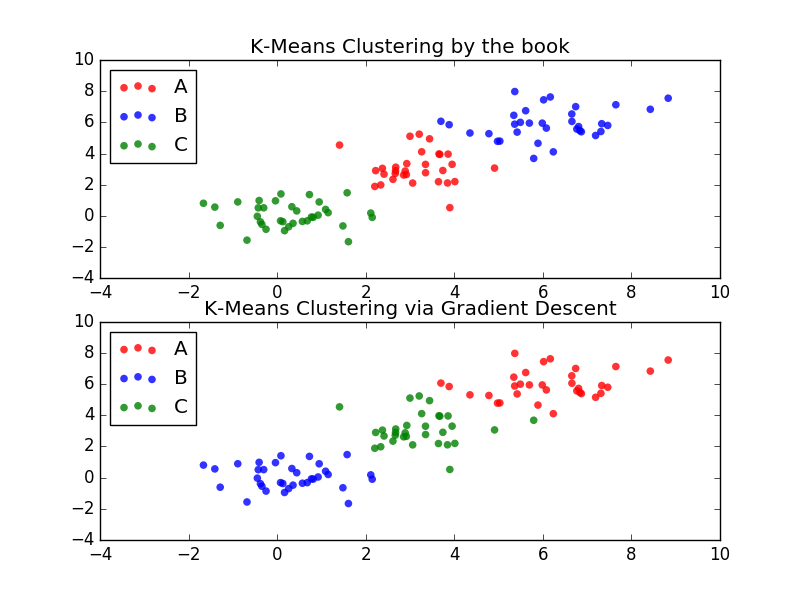
\includegraphics[width=0.7\textwidth]{imgs/gd_clust_good_attempt.png}
\caption{\label{fig:gd_clust_good} Example of a successful K-means clustering via Gradient Descent over the logits of cluster membership probabilities.}
\end{figure}
\section{Experiments with synthetic data}
\subsection{Learning a linear projection}
In this subsection we describe our experiments with learning the parameters of a simple embedding function, namely a linear projection $f:\R^n \rightarrow \R$, whose parameters should be learned.\\
The performance of an end-to-end clustering algorithm relies on many design choices and factors, and how they relate to the specific problem at hand.\\
In our experiments we examined the following factors:\\
\begin{itemize}
\item Clustering algorithm to be unrolled.  
\item Number of iterations which the clustering algorithm performs.
\item Various clusterer-specific hyperparameters, such as the bandwidth for the EM-clusterer, and the learn-rate and decrease schedule for the Differentiable-K-Means. 
\end{itemize}
We examined these and related factors on the following synthetic data sets:\\
I) Co-linear Gaussian Clusters\\
In this data set, the data is simply generated by a mixture of Gaussians, whose means are co-linear. The cluster membership for the data points correspond to the Gaussians which they are sampled from. \\
The Gaussians in this data set have isotopic covariance matrices, and since their means are co-linear, we know that the optimal linear projection parameters should be proportional to the parameters of the line which connects the Gaussians means.\\ % explain why this is the best?
An example for $n=3$ is portrayed at Figure x.\\
Anecdote: If you learn a linear projection for the ambiguous gaussians (placed at $10*unit_square$) plus a scaling factor, then using the EM clusterer, the scaling factor is pushed down. If you shrink the data by 0.1, the scale factor is pushed up. It stops changing at about $0.2$ times original data. why is that so?
\begin{comment}
\begin{figure}[h]
\begin{subfigure}{0.5\textwidth}
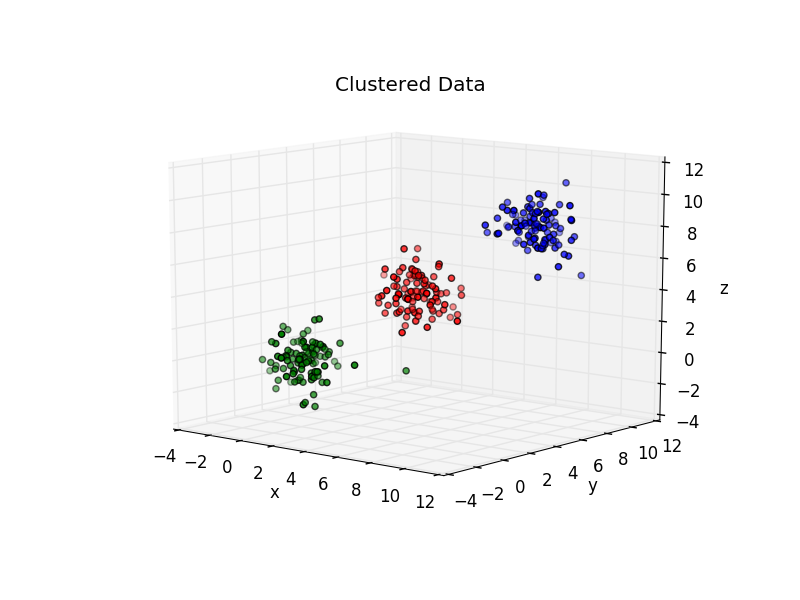
\includegraphics[width=0.9\linewidth, height=5cm]{imgs/figure_2.png} 
\caption{Co-Linear Gaussians}
\label{fig:subim1}
\end{subfigure}
\begin{subfigure}{0.5\textwidth}
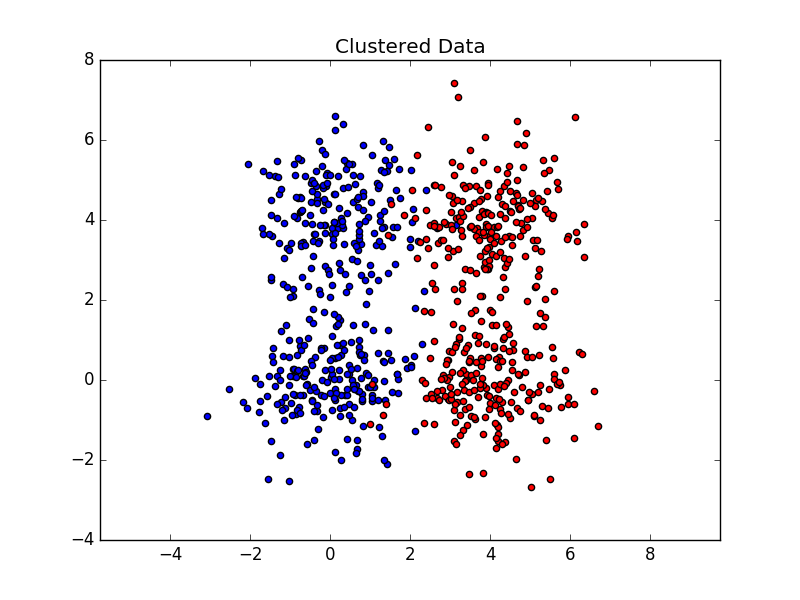
\includegraphics[width=0.9\linewidth, height=5cm]{imgs/ambiguous.png}
\caption{Ambiguous Gaussians}
\label{fig:subim2}
\end{subfigure}
\caption{Caption for this figure with two images}
\label{fig:image2}
\end{figure}
 \end{comment}
II) Ambiguous Gaussians % should a different term be used?

\section{Experiments With Real-World Data}
\subsection{Datasets}
\subsection{Experimental Protocol}
\subsection{Model Selection}

\begin{comment}
meow
\end{comment}
step 0: show that init 2 still outperforms other inits. we have plot for this
at first we checked which lr's are ok for the training to converge. this led us to 1e-5,1e-6.
% data for next paragraph in dir first_try
then we checked which bandwith params to use. at first we did this with lr=1e-5. this showed overfitting.
later we tried with lr=1e-6, which did not result in overfitting. this is interesting- shows a qualitative difference in models.

%when checking bw selection for lr=1e-6, we see that best gumbel temp and softmin_bw are 1. we dont have an upper bound yet on what seems a reasonable em_bw, so we check with additional experiments
%these experiments show that bw=1 seems best.
%What happens when we combine these different choices together?
%(show adhoc vs new bw)
%It seems it actually performs worse on generalization.
%Let's take the combination which performed best?
%combination of those performed best on miniTrue doesnt perform good on miniFalse 
combination of those performed best on miniTrue doesnt perform good on miniTrue 
%I now check miniFalse for all bw=1 (already checked) and all argmax for different bw. if this goes ok i enter this to miniTrue
% argmax on miniTrue is best on miniFalse
%Lets use the argmax then. that is when softmin_bw = 1, and the rest is the same
Now lets give it a total run with nmi loss as well
\subsection{Implementation Details}
\subsection{Results}
\subsection{General Details}
Following the experiments described at zemel17 song16, we test our approach on three known datasets:\\
\begin{itemize}
\item Caltech-UCSD Birds 200 \cite{WahCUB_200_2011}
\item Stanford Cars Dataset
\item Stanford Products Dataset
\end{itemize}
Each dataset consists of images which come from some shared context (i.e images of birds, cars or consumer products). The images in each dataset are further categorized into classes (E.g "Laysan Albatross" for birds, "2012 Tesla Model S" for cars, etc.) where images in the same class are considered semantically similar.
We split the datasets to a train and test set according to the splits described in Zemel17,Song16. At train time, mini-batches of images are sampled, and a clustering matrix over the sampled images is predicted. The $L_2$ difference between the prediction and the ground-truth matrix is used cost function.\\
The code for our experiments was written in Tensorflow \cite{greenwade93} version 1.8.0. A link to the publicly available git repository is listed below.\footnote{Link: \url{https://github.com/DanielCarmon/msc_project}}
\subsubsection{Depth of K-Means unrolling}
In our experiments different unroll depths $T\in\{1,3,5,10\}$ are tested. In the case where $T=1$, we simply output $BB^t$ as the prediction, where $B\in\mathbb{R}^n,k$ is the belief matrix for when the centroids are those initially sampled by the differentiable centroid sampling module described above. 
In the results section it is seen that deeper doesn't necessarily mean better, and that usually there is a "sweetspot", or optimal unroll depth $T$ for learning through K-Means optimization.

\subsubsection{Embedding Function}
As an embedding function $f:D\rightarrow \mathbb{R}^d$, we use the Inception-v3 \cite{greenwade93} architecture, with parameters pre-trained on the ImageNet\cite{greenwade93} dataset. As in Zemel17, song16, we removed the softmax operation at the last layer of the network, and added a linear layer. The output dimentionality $d$ of our linear layer is set to be the number of train classes for the first two datasets, and $512$ for the Products dataset, where the number of train classes is larger than $10^4$.\\

\subsubsection{Training Details}
% general pipeline
At train time we use batches of $n=100$ images per update step, with a ground-truth clustering matrix $Y\in R^{n,n}$. These images are sampled from $k\in{\{5,10,20\}}$ different classes, with each class contributing $n/k$ images to the batch. The $k$ class indices too are sampled at each iteration from a pool of classes whose images constitute the train data. Results for different values of $k$ are shown below.\\
% trajectory gradients
When training with differentiable clusterers that have intermediate beliefs (i.e when the unroll depth of the clusterer is greater than $1$), we use "auxillary gradients" by adding the loss for intermediate beliefs to the loss function we optimize over. This trick appears in previous deep learning works as well. E.g in \cite{greenwade93}, where the original Inception-v3 network was trained on ImageNet, "auxillary classifier" layers are maintained at train time, and their loss is added to the total loss function of the network. At test time, these classifiers are discarded. Using these "auxillary gradients" in our case favors embeddings who's clustering under K-Means++ doesn't just converges to a good local optima, but also does so quickly. Another way in which this trick benefits the training process is that it helps to alleviate the vanishing gradient problem\cite{greenwade93}, which occurs as unroll depth is increased.\\ % does it really occur?
Data pre-processing was done in the following way. Each image was first reshaped to shape $[299,299,3]$, in order to fit the Inception network's fixed input size. Afterwards the pixel intensities of each image were linearly scaled to $[0,1]$. For data augmentation, we used a single horizontal flip per image.\\
The following hyperparameters were used in our experiments. The bandwidth for the softmax at the differentiable clusterer's E-step is $1e-1$. We used the Adam \cite{} optimizer with a base learn rate of $1e-6$ to train the deep network's parameters.
We trained our models for $5e+4$ steps, which on a standard work station with a 3GHz 16-Core PC with 125GB RAM and a GeForce GTX TITAN X GPU with 13GB RAM took about 1 day to complete. 
\subsubsection{Testing Details}
At test time, the embedding function learned during training is used to embed the test data. 
The original (i.e non-differentiable) K-Means++ algorithm is then used to cluster the embedded test data, and the Normalized Mutual Information (NMI) \cite{greenwade93} is then used as a difference measure between the K-Means++ clustering over the embedded data and the ground-truth clustering.\\
In our experiments we used $\it{sklearn}$'s \cite{greenwade93} implementation for K-means++.
We tested the K-Means++ clustering every 100 parameter updates, in order to see how the NMI score for the learned embedding changes across training. We present results for the train data and the test data. % should we?
In the first two datasets, the classes in the train and test data are disjoint, although coming from a shared context (all being images of birds or cars). In the third dataset (Stanford Products), where an average class has about $5.3$ images, some classes occur in both data splits and some don't. In all cases, the learner must be able to generalize from classes seen during training to previously unseen classes. 

\subsection{CUB Dataset}
The CUB Dataset is comprised of 200 classes of different birds. Each class contains about 60 instances belonging to a single species. We sp lit the data to have the first 100 classes (5,864 images) for training, and the last 100 classes (5,924 images) for testing.
\subsubsection{Training Details}
...
\subsubsection{Results}
After every 100 parameter updates, we tested how well can the newly represented data be clustered, both for the train data and the test."Goodness of clustering" was measured via normalized mutual information. The following table shows both for train and test data how close with regard to ground truth were the new representations clustered.\\
\begin{figure}[h!]
\centering
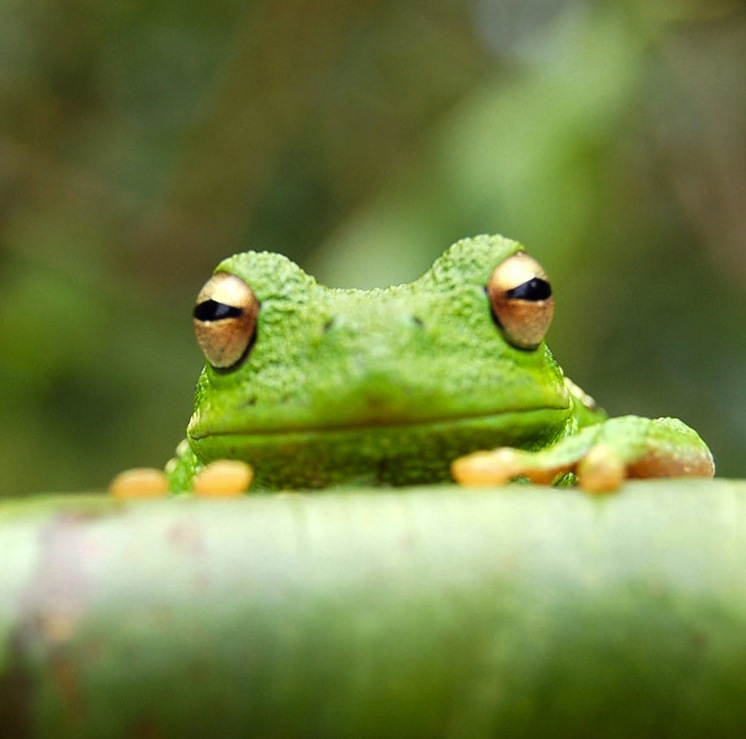
\includegraphics[width=0.3\textwidth]{imgs/frog.jpg}
\caption{\label{fig:frog}placeholder for image.}
\end{figure}
TODO: Add image that shows this. When done doing design choices elimination, train the best.
The following table summarizes the NMI score of previous benchmarks with addition to ours:
\begin{table}[h!]
\centering
\begin{tabular}{l|r}
Method & NMI \\\hline
Triplet s.h. (Schroff et al., 2015) & 55.38 \\
Lifted struct. (Song et al., 2016) & 56.50 \\
Npairs (Sohn, 2016) & 57.24 \\
Facility loc.(Song et al., 2017) & 59.23 \\
Spectral clust. (Zemel et al., 2017) & 59.16 \\
Ours & 60+ 
\end{tabular}
\caption{\label{tab:score compare} NMI evaluation on the Birds (CUB-200-
2011) dataset.}
\end{table}
\subsection{Stanford Cars Dataset}
Description of dataset goes here
\subsubsection{Training Details}
\subsubsection{Results}
\subsection{Ablation Studies}
We perform the following ablation studies on the Caltech-UCSD Birds-200-2011 dataset. We measure the NMI score of different variations in the architecture we proposed above. The variations we examined are difference in depth of the clustering inference module (i.e, how many belief update iterations occurred) and difference in number of clusters per training batch (i.e, how many bird categories where seen during each training iteration). There are existing trade-offs for each of these design choices. A deeper clustering inference module will give more accurate results, but may dilute the gradient signal such that learning is dampened. For the number of clusters per batch, a high number of seen categories in each batch may help reach a representation which will generalize (see discussion on ZSL in \ref{e2e_rep_learn}) better, yet on the other hand a too high number of categories will emphasize intra-cluster differences, while at the extreme end (when $k=n$) the supervision signal is degenerated to simply be the identity matrix. For both these design choice dimensions it seems from the following ablation studies that there is a "sweet-spot" somewhere between the extreme values. The variation which reached the highest NMI score over the test data isn't the model that was suggested by evaluating the different variation's clustering over the first 100 categories, and thus we did not report it's score (~0.62 NMI) when comparing our approach to other works. 

\iffalse
\begin{figure}[h!]
\centering
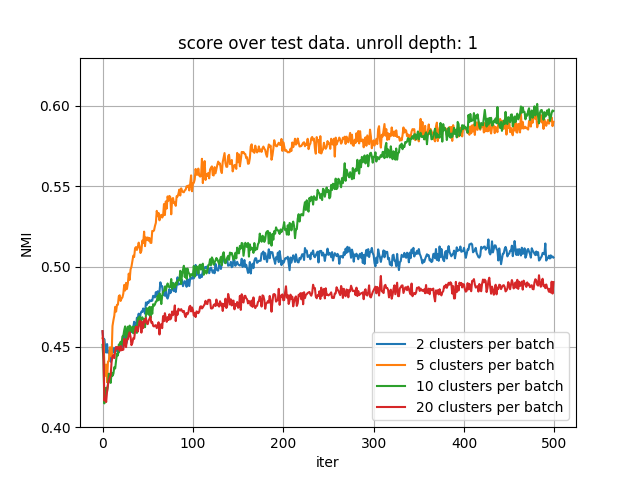
\includegraphics[width=1\textwidth]{imgs/cub_test_500/square/depth1.png}
\caption{\label{fig:cub_test_500} NMI Test scores for architecture with single belief update step.}
\end{figure}
\begin{figure}[h!]
\centering
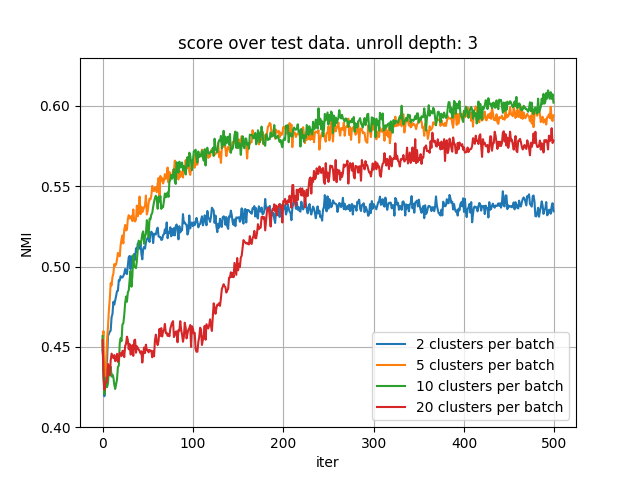
\includegraphics[width=1\textwidth]{imgs/cub_test_500/square/depth3.png}
\caption{\label{fig:cub_test_500} NMI Test scores for architecture with three belief update steps.}
\end{figure}
\begin{figure}[h!]
\centering
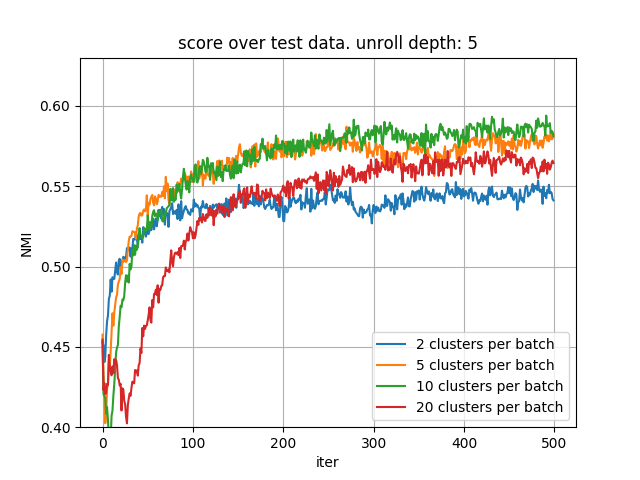
\includegraphics[width=1\textwidth]{imgs/cub_test_500/square/depth5.png}
\caption{\label{fig:cub_test_500} NMI Test scores for architecture with five belief update steps.}
\end{figure}
\begin{figure}[h!]
\centering
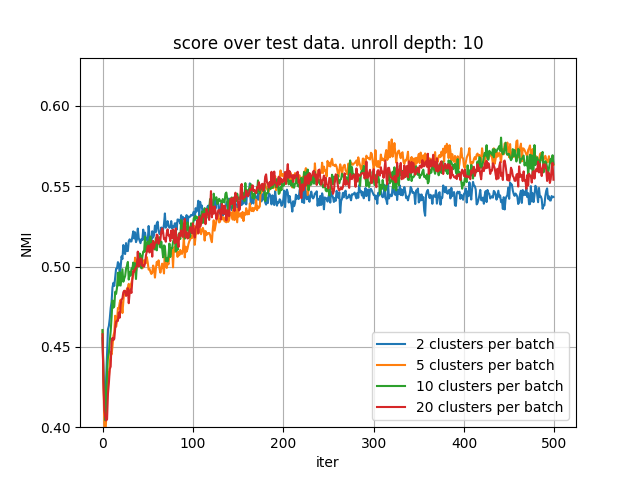
\includegraphics[width=1\textwidth]{imgs/cub_test_500/square/depth10.png}
\caption{\label{fig:cub_test_500} NMI Test scores for architecture with ten belief update steps.}
\end{figure}
\begin{figure}[h!]
\centering
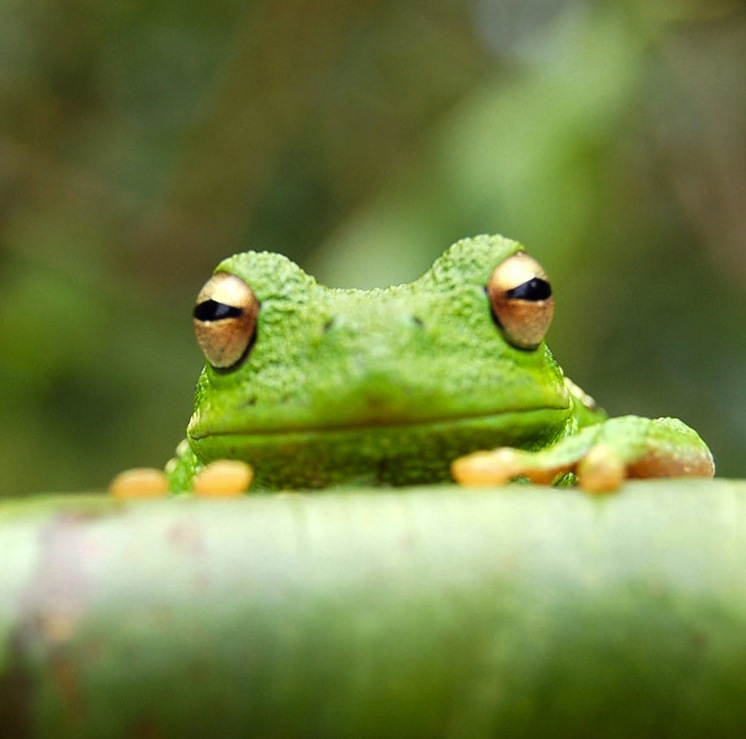
\includegraphics[width=0.3\textwidth]{imgs/frog.jpg}
\caption{\label{fig:frog}placeholder for image.}
\end{figure}
TODO: Add image that shows this. When done doing design choices elimination, train the best.
The following table summarizes the NMI score of previous benchmarks with addition to ours:
\begin{table}[h!]
\centering
\begin{tabular}{l|r}
Method & NMI \\\hline
Triplet s.h. (Schroff et al., 2015) & 53.35 \\
Lifted struct (Song et al., 2016) & 56.88 \\
Npairs (Sohn, 2016) & 57.79 \\ 
Facility loc. (Song et al., 2017) & 59.04 \\
Spectral clust. (Zemel et atl., 2017) & 64.25 \\
\end{tabular}
\caption{\label{tab:score compare} NMI and Recall@K evaluation on the Cars196 dataset.}
\end{table}
\subsection{Stanford Products Dataset}
Description of dataset goes here
\subsubsection{Training Details}
\subsubsection{Results}
\begin{figure}[h!]
\centering
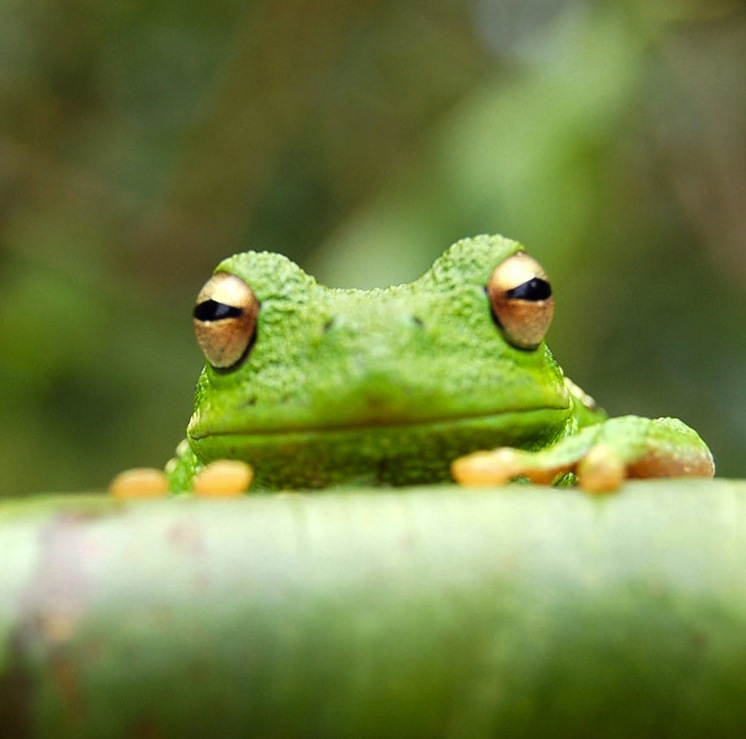
\includegraphics[width=0.3\textwidth]{imgs/frog.jpg}
\caption{\label{fig:frog}placeholder for image.}
\end{figure}
TODO: Add image that shows this. When done doing design choices elimination, train the best.
The following table summarizes the NMI score of previous benchmarks with addition to ours:
\begin{table}[h!]
\centering
\begin{tabular}{l|r}[h!]
Method & NMI \\\hline
Triplet s.h. (Schroff et al., 2015) & 89.46 \\
Lifted struct. (Song et al., 2016) & 88.65 \\
Npairs (Sohn, 2016) & 89.37 \\
Facility loc.(Song et al., 2017) & 89.48 \\
Spectral clust. (Zemel et al., 2017) &  89.40 \\
Ours & ?
\end{tabular}
\caption{\label{tab:score compare} NMI evaluation on the Products (Stanford
Online Products) dataset.}
\end{table}


\begin{comment}
\subsubsection{Effect of Unrolling Depth}
\subsubsection{Effect of Centroid Initialization Method}
\begin{figure}[h!]
\centering
\includegraphics[width=0.3\textwidth]{centroid_init_comparison.png}
\caption{\label{fig:init_comparison} Comparison of NMI scores when trained using different centroid initialization methods.}
\end{figure}
\end{comment}

\fi
